\begin{adjustbox}{width=\textwidth}
	\begin{tikzpicture}[every node/.style={inner sep=0,outer sep=0}]
	
		\node [anchor=north east] (imgSpalten) at (-0.03\textwidth,0) {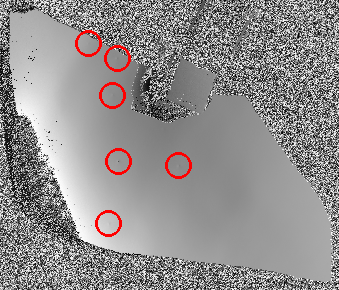
\includegraphics[width=.47\textwidth]{04_deflektometrischeRegistrierung/auswertungDeflektometrischeRegistrierung/figures/pickelDeflektometrischeRegistrierung}};
		\node [below=0.2cm of imgSpalten] {Graubild der Spaltenzuordnung \acrshort{frx}$(x,y)$};
		\node [anchor=north west] (imgGradienten) at (0.03\textwidth,0) {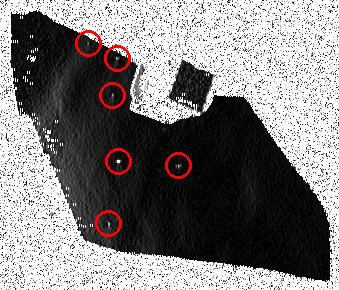
\includegraphics[width=.47\textwidth]{04_deflektometrischeRegistrierung/auswertungDeflektometrischeRegistrierung/figures/pickelGradientenbild}};
		\node [below=0.2cm of imgGradienten, align = center] {Gradientenbild von \acrshort{frx}$(x,y)$ über den \\ Sobel-Operator in $x$-Richtung};
		
	\end{tikzpicture}
\end{adjustbox}
\caption[Hervorhebung von Pickeln auf reflektierenden Oberflächen.]{Deflektometrische Spaltenregistrierung eines spiegelnden Porzellanbruch\-stücks und das Gradientenbild.}